\clearpage
\section{Weight averaging versus functional ensembling}%
\label{app:wa_vs_ens_analysis}%
\begin{wrapfigure}[12]{hR!}{0.34\textwidth}
    \vspace{-3em}%
    \centering%
    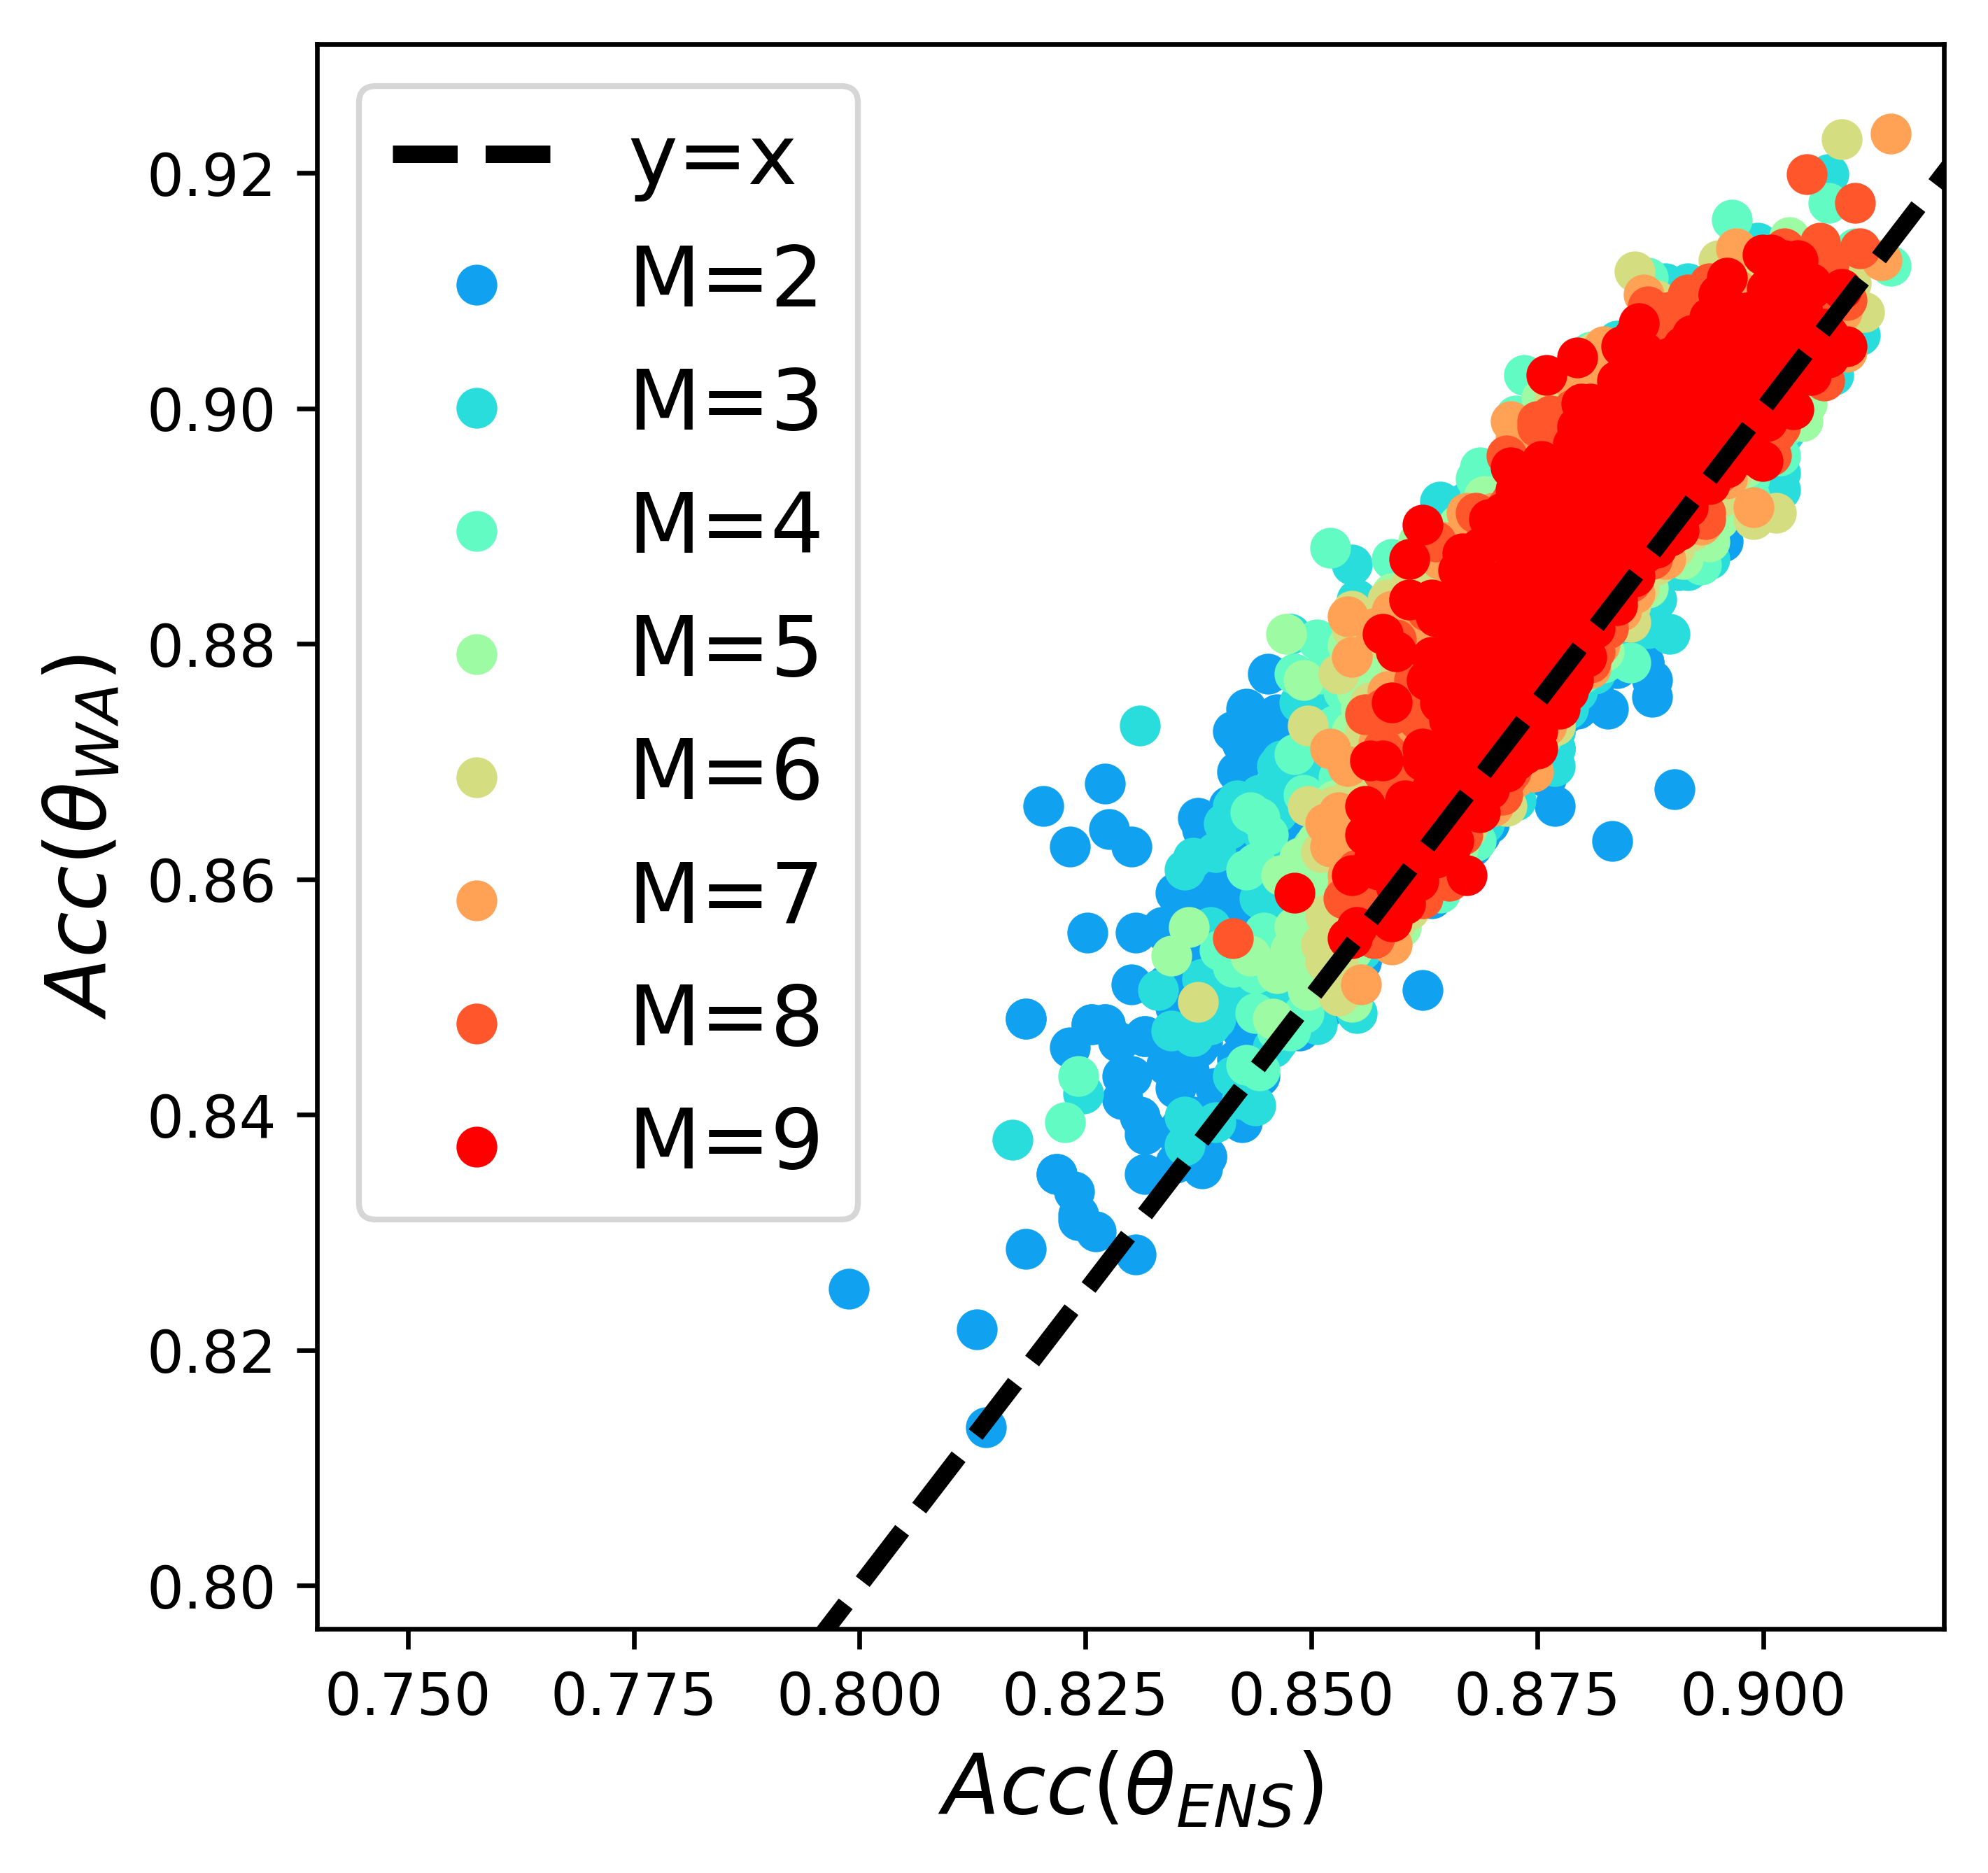
\includegraphics[width=0.34\textwidth]{pictures/files/final/pacs0_samediffruns210_ens_wa.png}%
    \caption{$f_{\text{WA}}$ performs similarly or better than $f_{\text{ENS}}$ on domain \enquote{Art} on PACS.}%
    \label{fig:pacs_samediffruns_ens210_soup}%
\end{wrapfigure}%
We further compare the following two methods to combine $M$ weights $\{\theta(l_S^{(m)})\}_{m=1}^M$: $f_{\text{WA}}$ that averages the weights and $f_{\text{ENS}}$ \cite{Lakshminarayanan2017} that averages the predictions.
We showed in \Cref{lemma:wa_ensembling} that $f_{\text{WA}} \approx f_{\text{ENS}}$ when $\max_{m=1}^{M}\| \theta(l_S^{(m)}) - \theta_{\text{WA}}\|_2$ is small.

In particular, when $\{l_S^{(m)}\}_{m=1}^M$ share the same initialization and the hyperparameters are sampled from mild ranges, we empirically validate our approximation on OfficeHome in \Cref{fig:home0_samediffruns_net_soup}. This is confirmed on PACS dataset in \Cref{fig:pacs_samediffruns_ens210_soup}.
For both datasets, we even observe that $f_{\text{WA}}$ performs slightly but consistently better than $f_{\text{ENS}}$. The observed improvement is non-trivial; we refer to Equation 1 in \cite{Wortsman2022ModelSA} for some initial explanations based on the value of \ood Hessian and the confidence of $f_{\text{WA}}$. The complete analysis of this second-order difference is left for future work.

Yet, we do not claim that $f_{\text{WA}}$ is systematically better than $f_{\text{ENS}}$.
In \Cref{table:db_home0_ensvsswa}, we show that this is no longer the case when we relax our two constraints, consistently with \Cref{fig:home0_locality_requirement}.
\textit{First}, when the classifiers' initializations vary, ENS improves thanks to this additional diversity; in contrast, DiWA degrades because weights are no longer averageable.
% As a side note, DiWA surprisingly remains better than ERM.
\textit{Second}, when the hyperparameters are sampled from extreme ranges (defined in \Cref{tab:hyperparam}), performance drops significantly for DiWA, but much less for ENS.
As a side note, the downward trend in this second setup (even for ENS) is due to inadequate hyperparameters that degrade the expected individual performances.

This highlights a limitation of DiWA, which requires weights that satisfy the locality requirement or are at least linearly connectable.
In contrast, Deep Ensembles \cite{Lakshminarayanan2017} are computationally expensive (and even impractical for large $M$), but can leverage additional sources of diversity.
An interesting extension of DiWA for future work would be to consider the functional ensembling of several DiWAs trained from different initializations or even with different network architectures \cite{singh2016swapout}.
Thus the Ensemble of Averages (EoA) strategy introduced in  \cite{arpit2021ensemble} is complementary to DiWA and could be extended into an Ensemble of Diverse Averages.

\begin{table}[h]%
    \caption{\textbf{DiWA's vs. ENS's accuracy ($\%, \uparrow$)} on domain \enquote{Art} from OfficeHome when varying initialization and hyperparameter ranges. Best on each setting is in \textbf{bold}.}
    \centering
    \adjustbox{width=1.0\textwidth}{
        \centering
        \begin{tabular}{ccc ccccc}
            \toprule
            \multicolumn{3}{c}{Configuration} & \multicolumn{2}{c}{\textbf{$M=20$}} && \multicolumn{2}{c}{\textbf{$M=60$}} \\
            \cmidrule(lr){0-2} \cmidrule(lr){4-5} \cmidrule(lr){7-8} Shared classifier init && Mild hyperparameter ranges & DiWA & ENS && DiWA & ENS \\
            \midrule
              \cmark          && \cmark    & \textbf{67.3} $\pm$ 0.2  & 66.1 $\pm$ 0.1 & & \textbf{67.7}    &   66.5      \\
            \xmark          && \cmark    & 65.0 $\pm$ 0.5  & \textbf{67.5} $\pm$ 0.3 & & 65.9     &  \textbf{68.5}      \\
            \cmark          && \xmark    & 56.6 $\pm$ 0.9  & \textbf{64.3} $\pm$ 0.4 & & 59.5     &  \textbf{64.7}      \\   

            % \midrule
            % \multirow{3}{*}{ENS} & \xmark           & \xmark    & 66.1 $\pm$ 0.1  & 66.5            \\
            %                                             & \cmark           & \xmark    & 67.5 $\pm$ 0.3  & \textbf{68.5}            \\
            %                                             & \xmark          & \cmark     & 64.3 $\pm$ 0.4  & \textbf{64.7}            \\
            \bottomrule
        \end{tabular}}
    \label{table:db_home0_ensvsswa}%
\end{table}



